
\documentclass[letterpaper,hide notes,xcolor={table,svgnames},pdftex,10pt]{beamer}
\def\showexamples{t}


%\usepackage[svgnames]{xcolor}

%% Demo talk
%\documentclass[letterpaper,notes=show]{beamer}

\usecolortheme{crane}
\setbeamertemplate{navigation symbols}{}

\usetheme{MyPittsburgh}
%\usetheme{Frankfurt}

%\usepackage{tipa}

\usepackage{hyperref}
\usepackage{graphicx,xspace}
\usepackage[normalem]{ulem}
\usepackage{multicol}
\usepackage{amsmath,amssymb,amsthm,graphicx,xspace}
\newcommand\SF[1]{$\bigstar$\footnote{SF: #1}}

\usepackage[default]{sourcesanspro}
\usepackage[T1]{fontenc}
\usepackage[scaled]{beramono}
\usepackage{tikzpagenodes}

\newcounter{tmpnumSlide}
\newcounter{tmpnumNote}


% old question code
%\newcommand\question[1]{{$\bigstar$ \small \onlySlide{2}{#1}}}
% \newcommand\nquestion[1]{\ifdefined \presentationonly \textcircled{?} \fi \note{\par{\Large \textbf{?}} #1}}
% \newcommand\nanswer[1]{\note{\par{\Large \textbf{A}} #1}}


 \newcommand\mnote[1]{%
   \addtocounter{tmpnumSlide}{1}
   \ifdefined\showcues {~\tiny\fbox{\arabic{tmpnumSlide}}}\fi
   \note{\setlength{\parskip}{1ex}\addtocounter{tmpnumNote}{1}\textbf{\Large \arabic{tmpnumNote}:} {#1\par}}}

\newcommand\mmnote[1]{\note{\setlength{\parskip}{1ex}#1\par}}

%\newcommand\mnote[2][]{\ifdefined\handoutwithnotes {~\tiny\fbox{#1}}\fi
% \note{\setlength{\parskip}{1ex}\textbf{\Large #1:} #2\par}}

%\newcommand\mnote[2][]{{\tiny\fbox{#1}} \note{\setlength{\parskip}{1ex}\textbf{\Large #1:} #2\par}}

\newcommand\mquestion[2]{{~\color{red}\fbox{?}}\note{\setlength{\parskip}{1ex}\par{\Large \textbf{?}} #1} \note{\setlength{\parskip}{1ex}\par{\Large \textbf{A}} #2\par}\ifdefined \presentationonly \pause \fi}

\newcommand\blackboard[1]{%
\ifdefined   \showblackboard
  {#1}
  \else {\begin{center} \fbox{\colorbox{blue!30}{%
         \begin{minipage}{.95\linewidth}%
           \hspace{\stretch{1}} Some space intentionally left blank; done at the blackboard.%
         \end{minipage}}}\end{center}}%
         \fi%
}



%\newcommand\q{\tikz \node[thick,color=black,shape=circle]{?};}
%\newcommand\q{\ifdefined \presentationonly \textcircled{?} \fi}

\usepackage{listings}
\lstset{basicstyle=\footnotesize\ttfamily,
	breaklines=true,
	aboveskip=15pt,
  	belowskip=15pt,
	frame=lines,
	numbers=left, basicstyle=\scriptsize, numberstyle=\tiny, stepnumber=0, numbersep=2pt
}

\usepackage{siunitx}
\newcommand\sius[1]{\num[group-separator = {,}]{#1}\si{\micro\second}}
\newcommand\sims[1]{\num[group-separator = {,}]{#1}\si{\milli\second}}
\newcommand\sins[1]{\num[group-separator = {,}]{#1}\si{\nano\second}}
\sisetup{group-separator = {,}, group-digits = true}

%% -------------------- tikz --------------------
\usepackage{tikz}
\usetikzlibrary{positioning}
\usetikzlibrary{arrows,backgrounds,automata,decorations.shapes,decorations.pathmorphing,decorations.markings,decorations.text,decorations.pathreplacing}

\tikzstyle{place}=[circle,draw=blue!50,fill=blue!20,thick, inner sep=0pt,minimum size=6mm]
\tikzstyle{transition}=[rectangle,draw=black!50,fill=black!20,thick, inner sep=0pt,minimum size=4mm]

\tikzstyle{block}=[rectangle,draw=black, thick, inner sep=5pt]
\tikzstyle{bullet}=[circle,draw=black, fill=black, thin, inner sep=2pt]

\tikzstyle{pre}=[<-,shorten <=1pt,>=stealth',semithick]
\tikzstyle{post}=[->,shorten >=1pt,>=stealth',semithick]
\tikzstyle{bi}=[<->,shorten >=1pt,shorten <=1pt, >=stealth',semithick]

\tikzstyle{mut}=[-,>=stealth',semithick]

\tikzstyle{treereset}=[dashed,->, shorten >=1pt,>=stealth',thin]

\usepackage{ifmtarg}
\usepackage{xifthen}
\makeatletter
% new counter to now which frame it is within the sequence
\newcounter{multiframecounter}
% initialize buffer for previously used frame title
\gdef\lastframetitle{\textit{undefined}}
% new environment for a multi-frame
\newenvironment{multiframe}[1][]{%
\ifthenelse{\isempty{#1}}{%
% if no frame title was set via optional parameter,
% only increase sequence counter by 1
\addtocounter{multiframecounter}{1}%
}{%
% new frame title has been provided, thus
% reset sequence counter to 1 and buffer frame title for later use
\setcounter{multiframecounter}{1}%
\gdef\lastframetitle{#1}%
}%
% start conventional frame environment and
% automatically set frame title followed by sequence counter
\begin{frame}%
\frametitle{\lastframetitle~{\normalfont(\arabic{multiframecounter})}}%
}{%
\end{frame}%
}
\makeatother

\makeatletter
\newdimen\tu@tmpa%
\newdimen\ydiffl%
\newdimen\xdiffl%
\newcommand\ydiff[2]{%
    \coordinate (tmpnamea) at (#1);%
    \coordinate (tmpnameb) at (#2);%
    \pgfextracty{\tu@tmpa}{\pgfpointanchor{tmpnamea}{center}}%
    \pgfextracty{\ydiffl}{\pgfpointanchor{tmpnameb}{center}}%
    \advance\ydiffl by -\tu@tmpa%
}
\newcommand\xdiff[2]{%
    \coordinate (tmpnamea) at (#1);%
    \coordinate (tmpnameb) at (#2);%
    \pgfextractx{\tu@tmpa}{\pgfpointanchor{tmpnamea}{center}}%
    \pgfextractx{\xdiffl}{\pgfpointanchor{tmpnameb}{center}}%
    \advance\xdiffl by -\tu@tmpa%
}
\makeatother
\newcommand{\copyrightbox}[3][r]{%
\begin{tikzpicture}%
\node[inner sep=0pt,minimum size=2em](ciimage){#2};
\usefont{OT1}{phv}{n}{n}\fontsize{4}{4}\selectfont
\ydiff{ciimage.south}{ciimage.north}
\xdiff{ciimage.west}{ciimage.east}
\ifthenelse{\equal{#1}{r}}{%
\node[inner sep=0pt,right=1ex of ciimage.south east,anchor=north west,rotate=90]%
{\raggedleft\color{black!50}\parbox{\the\ydiffl}{\raggedright{}#3}};%
}{%
\ifthenelse{\equal{#1}{l}}{%
\node[inner sep=0pt,right=1ex of ciimage.south west,anchor=south west,rotate=90]%
{\raggedleft\color{black!50}\parbox{\the\ydiffl}{\raggedright{}#3}};%
}{%
\node[inner sep=0pt,below=1ex of ciimage.south west,anchor=north west]%
{\raggedleft\color{black!50}\parbox{\the\xdiffl}{\raggedright{}#3}};%
}
}
\end{tikzpicture}
}


%% --------------------

%\usepackage[excludeor]{everyhook}
%\PushPreHook{par}{\setbox0=\lastbox\llap{MUH}}\box0}

%\vspace*{\stretch{1}

%\setbox0=\lastbox \llap{\textbullet\enskip}\box0}

\setlength{\parskip}{\fill}

\newcommand\noskips{\setlength{\parskip}{1ex}}
\newcommand\doskips{\setlength{\parskip}{\fill}}

\newcommand\xx{\par\vspace*{\stretch{1}}\par}
\newcommand\xxs{\par\vspace*{2ex}\par}
\newcommand\tuple[1]{\langle #1 \rangle}
\newcommand\code[1]{{\sf \footnotesize #1}}
\newcommand\ex[1]{\uline{Example:} \ifdefined \presentationonly \pause \fi
  \ifdefined\showexamples#1\xspace\else{\uline{\hspace*{2cm}}}\fi}

\newcommand\ceil[1]{\lceil #1 \rceil}


\AtBeginSection[]
{
   \begin{frame}
       \frametitle{Outline}
       \tableofcontents[currentsection]
   \end{frame}
}



\pgfdeclarelayer{edgelayer}
\pgfdeclarelayer{nodelayer}
\pgfsetlayers{edgelayer,nodelayer,main}

\tikzstyle{none}=[inner sep=0pt]
\tikzstyle{rn}=[circle,fill=Red,draw=Black,line width=0.8 pt]
\tikzstyle{gn}=[circle,fill=Lime,draw=Black,line width=0.8 pt]
\tikzstyle{yn}=[circle,fill=Yellow,draw=Black,line width=0.8 pt]
\tikzstyle{empty}=[circle,fill=White,draw=Black]
\tikzstyle{bw} = [rectangle, draw, fill=blue!20, 
    text width=4em, text centered, rounded corners, minimum height=2em]
    
    \newcommand{\CcNote}[1]{% longname
	This work is licensed under the \textit{Creative Commons #1 3.0 License}.%
}
\newcommand{\CcImageBy}[1]{%
	\includegraphics[scale=#1]{creative_commons/cc_by_30.pdf}%
}
\newcommand{\CcImageSa}[1]{%
	\includegraphics[scale=#1]{creative_commons/cc_sa_30.pdf}%
}
\newcommand{\CcImageNc}[1]{%
	\includegraphics[scale=#1]{creative_commons/cc_nc_30.pdf}%
}
\newcommand{\CcGroupBySa}[2]{% zoom, gap
	\CcImageBy{#1}\hspace*{#2}\CcImageNc{#1}\hspace*{#2}\CcImageSa{#1}%
}
\newcommand{\CcLongnameByNcSa}{Attribution-NonCommercial-ShareAlike}

\newenvironment{changemargin}[1]{% 
  \begin{list}{}{% 
    \setlength{\topsep}{0pt}% 
    \setlength{\leftmargin}{#1}% 
    \setlength{\rightmargin}{1em}
    \setlength{\listparindent}{\parindent}% 
    \setlength{\itemindent}{\parindent}% 
    \setlength{\parsep}{\parskip}% 
  }% 
  \item[]}{\end{list}} 




\title{Lecture 6 --- Working with Threads }

\author{Patrick Lam \& Jeff Zarnett \\ \small \texttt{patrick.lam@uwaterloo.ca} \texttt{jzarnett@uwaterloo.ca}}
\institute{Department of Electrical and Computer Engineering \\
  University of Waterloo}
\date{\today}


\begin{document}

\begin{frame}
  \titlepage

 \end{frame}


%%%%%%%%%%%%%%%%%%%%%%%%%%%%%%%%%%%%%%%%%%%%%%%%%%%%%%%%%%%%%%%%%%%%%%%%%%%%%%%%

\begin{frame}
  \frametitle{POSIX Threads}


  \begin{itemize}
    \item Available on most systems
    \vfill
    \item Windows has pthreads Win32, but I wouldn't use it; \\use Linux for
          this course
    \vfill
    \item API available by {\tt \#include <pthread.h>}
    \vfill
    \item Compile with pthread flag \\ ({\tt gcc -pthread prog.c -o prog})
  \end{itemize}

\end{frame}



\begin{frame}[fragile]
\frametitle{Pthread Functions}

Need a refresher? See the pthreads.pdf document in the course repository!

\begin{lstlisting}[language=C]
pthread_create( pthread_t *thread, const pthread_attr_t *attributes,
                void *(*start_routine)( void * ), void *argument )
pthread_join( pthread_t thread, void **return_value )
pthread_detach( pthread_t thread )
pthread_cancel( pthread_t thread )
pthread_testcancel( ) /* If the thread is cancelled, this function does not return (thread terminated) */
pthread_exit( void *value )
\end{lstlisting}


\end{frame}

%%%%%%%%%%%%%%%%%%%%%%%%%%%%%%%%%%%%%%%%%%%%%%%%%%%%%%%%%%%%%%%%%%%%%%%%%%%%%%%%

\begin{frame}[fragile]
  \frametitle{C++ 11 Threads}


  \begin{itemize}
    \item Now part of the C++ standard (library)
    \vfill
    \item API available with {\tt \#include <thread>}
    \vfill
    \item Compile with flags: \\ (\verb!g++ -std=c++11 -pthread prog.c -o prog!)
  \end{itemize}

\end{frame}

%%%%%%%%%%%%%%%%%%%%%%%%%%%%%%%%%%%%%%%%%%%%%%%%%%%%%%%%%%%%%%%%%%%%%%%%%%%%%%%%
\begin{frame}[fragile]
  \frametitle{Creating Threads---C++11 Example}


\begin{lstlisting}[language=C]
#include <thread>
#include <iostream>

void run() {
  std::cout << "In run\n";
}

int main() {
  std::thread t1(run);
  std::cout << "In main\n";
  t1.join(); // hang in there...
}
\end{lstlisting}

\end{frame}
%%%%%%%%%%%%%%%%%%%%%%%%%%%%%%%%%%%%%%%%%%%%%%%%%%%%%%%%%%%%%%%%%%%%%%%%%%%%%%%%


\begin{frame}
\frametitle{Attributes}

 In previous courses, the default attributes were fine...
 
 But now we should know about them!
 
 \begin{center}
 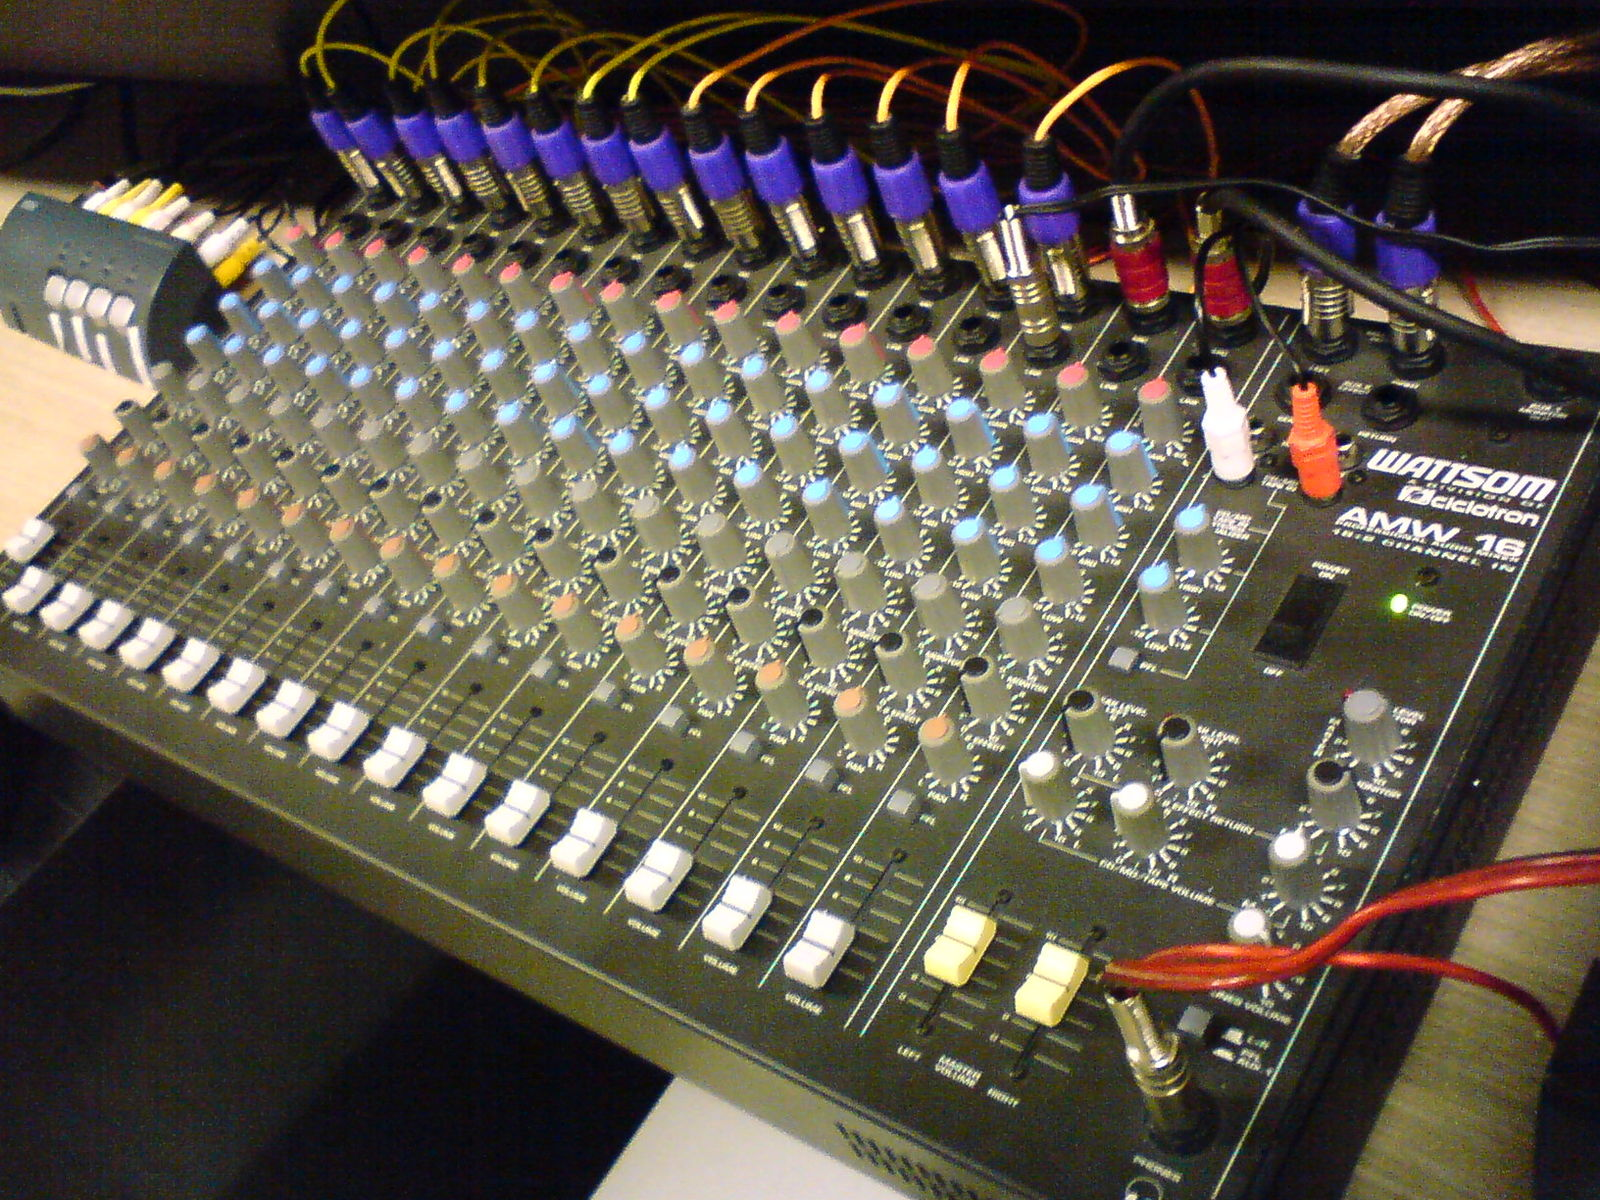
\includegraphics[width=0.8\textwidth]{images/mixing-console.jpg}
 \end{center}

\end{frame}



%%%%%%%%%%%%%%%%%%%%%%%%%%%%%%%%%%%%%%%%%%%%%%%%%%%%%%%%%%%%%%%%%%%%%%%%%%%%%%%%
\begin{frame}
  \frametitle{Attributes}


  By default, threads are {\it joinable} on Linux, but a more portable way to
  know what you're getting is to set thread attributes. You can change:
  \begin{itemize}
    \item Detached or joinable state
    \item Scheduling inheritance
    \item Scheduling policy
    \item Scheduling parameters
    \item Scheduling contention scope
    \item Stack size
    \item Stack address
    \item Stack guard (overflow) size
  \end{itemize}


\end{frame}
%%%%%%%%%%%%%%%%%%%%%%%%%%%%%%%%%%%%%%%%%%%%%%%%%%%%%%%%%%%%%%%%%%%%%%%%%%%%%%%%

%%%%%%%%%%%%%%%%%%%%%%%%%%%%%%%%%%%%%%%%%%%%%%%%%%%%%%%%%%%%%%%%%%%%%%%%%%%%%%%%
\begin{frame}[fragile]
  \frametitle{Attributes---Example}


  \begin{lstlisting}[language=C]
size_t stacksize;
pthread_attr_t attributes;
pthread_attr_init(&attributes);
pthread_attr_getstacksize(&attributes, &stacksize);
printf("Stack size = %i\n", stacksize);
pthread_attr_destroy(&attributes);
  \end{lstlisting}
Running this on a laptop produces:
  \begin{lstlisting}
jon@riker examples master % ./stack_size 
Stack size = 8388608
  \end{lstlisting}
  Setting a thread state to joinable:
  \begin{lstlisting}
pthread_attr_setdetachstate(&attributes,
                            PTHREAD_CREATE_JOINABLE);
  \end{lstlisting}


\end{frame}
%%%%%%%%%%%%%%%%%%%%%%%%%%%%%%%%%%%%%%%%%%%%%%%%%%%%%%%%%%%%%%%%%%%%%%%%%%%%%%%%

%%%%%%%%%%%%%%%%%%%%%%%%%%%%%%%%%%%%%%%%%%%%%%%%%%%%%%%%%%%%%%%%%%%%%%%%%%%%%%%%
\begin{frame}[fragile]
  \frametitle{Passing Data to Pthreads threads\ldots Wrongly}


Consider this snippet:
\vfill
\begin{lstlisting}[language=C]
int i;
for (i = 0; i < 10; ++i)
  pthread_create(&thread[i], NULL, run, (void*)&i);
\end{lstlisting}
  \vfill
  This is a \alert{terrible} idea. Why?
  \vfill
  \begin{enumerate}
    \item<2-> The value of {\tt i} will probably change before the thread executes
    \item<2-> The memory for {\tt i} may be out of scope, and therefore invalid by
          the time the thread executes
  \end{enumerate}


\end{frame}
%%%%%%%%%%%%%%%%%%%%%%%%%%%%%%%%%%%%%%%%%%%%%%%%%%%%%%%%%%%%%%%%%%%%%%%%%%%%%%%%

%%%%%%%%%%%%%%%%%%%%%%%%%%%%%%%%%%%%%%%%%%%%%%%%%%%%%%%%%%%%%%%%%%%%%%%%%%%%%%%%
\begin{frame}[fragile]
  \frametitle{Passing Data to Pthreads threads}
  
Correct:


\begin{lstlisting}[language=C]
int i;
int*
for (i = 0; i < 10; ++i) {
  arg = malloc( sizeof( int ) );
  *arg = i;
  pthread_create(&thread[i], NULL, run, arg);
}
\end{lstlisting}


\end{frame}
%%%%%%%%%%%%%%%%%%%%%%%%%%%%%%%%%%%%%%%%%%%%%%%%%%%%%%%%%%%%%%%%%%%%%%%%%%%%%%%%



\begin{frame}[fragile]
\frametitle{\texttt{int*} and \texttt{int} are always the same size, right guys?}

What about:
\begin{lstlisting}[language=C]
int i;
for (i = 0; i < 10; ++i)
  pthread_create(&thread[i], NULL, run, (void*)i);

...

void* run(void* arg) {
  int id = (int)arg;
\end{lstlisting}
  \vfill
  This is suggested in the book, but should carry a warning:

  \vfill
  \begin{itemize}
    \item<2-> Beware size mismatches between arguments: 
      no guarantee that a pointer is the same size as an int, so your data
      may overflow.
    \item<2-> Sizes of data types change between systems. For maximum
      portability, just use pointers you got {\tt from malloc}.
  \end{itemize}


\end{frame}

%%%%%%%%%%%%%%%%%%%%%%%%%%%%%%%%%%%%%%%%%%%%%%%%%%%%%%%%%%%%%%%%%%%%%%%%%%%%%%%%
\begin{frame}[fragile]
  \frametitle{Detached Threads}


  {\it Joinable} threads (the default) wait for someone to call
  {\tt pthread\_join} before they release their resources.
  \vfill
  {\it Detached} threads release their resources when they terminate, without
  being joined.
  \vfill
  \begin{lstlisting}[language=C]
int pthread_detach(pthread_t thread);
  \end{lstlisting}
  \vfill
  {\bf thread}: marks the thread as detached
  \vfill
  returns 0 on success, error number otherwise.
  \vfill
  Calling {\tt pthread\_detach} on an already detached thread results in undefined
  behaviour.


\end{frame}
%%%%%%%%%%%%%%%%%%%%%%%%%%%%%%%%%%%%%%%%%%%%%%%%%%%%%%%%%%%%%%%%%%%%%%%%%%%%%%%%


%%%%%%%%%%%%%%%%%%%%%%%%%%%%%%%%%%%%%%%%%%%%%%%%%%%%%%%%%%%%%%%%%%%%%%%%%%%%%%%%
\begin{frame}[fragile]
  \frametitle{Passing Data to C++11 threads}

It's easier to get data to threads in C++11:
\begin{lstlisting}[language=C]
#include <thread>
#include <iostream>

void run(int i) {
  std::cout << "In run " << i << "\n";
}

int main() {
  for (int i = 0; i < 10; ++i) {
    std::thread t1(run, i);
    t1.detach();.
  }
}
\end{lstlisting}

  
\end{frame}
%%%%%%%%%%%%%%%%%%%%%%%%%%%%%%%%%%%%%%%%%%%%%%%%%%%%%%%%%%%%%%%%%%%%%%%%%%%%%%%%


\begin{frame}
\frametitle{Thread Safety}

Make sure the libraries you use are  \alert{thread-safe}.

That means it protects its shared data (more detail later).

``How do I know?''

Well, you could... Read the documentation...?


\end{frame}


\begin{frame}
\frametitle{READ THE WHAT?!}

\begin{center}
	
\includegraphics[width=0.5\textwidth]{images/meatloaf.jpeg}
\end{center}

\end{frame}



%%%%%%%%%%%%%%%%%%%%%%%%%%%%%%%%%%%%%%%%%%%%%%%%%%%%%%%%%%%%%%%%%%%%%%%%%%%%%%%%
\begin{frame}
  \frametitle{Thread Safety}

glibc reentrant functions are also safe.

A program can have more than one thread calling these functions concurrently.
   
{\bf Example:} {\tt rand\_r} versus {\tt rand}.

\end{frame}
%%%%%%%%%%%%%%%%%%%%%%%%%%%%%%%%%%%%%%%%%%%%%%%%%%%%%%%%%%%%%%%%%%%%%%%%%%%%%%%%


\begin{frame}
\frametitle{Joinable Threads and Detached Threads}

Joinable threads hang around until someone joins them.

Detached threads clean up as soon as execution is finished.

It is good practice to detach threads if they are never joined.

And undefined behaviour to try to join a detached thread.

\end{frame}



%%%%%%%%%%%%%%%%%%%%%%%%%%%%%%%%%%%%%%%%%%%%%%%%%%%%%%%%%%%%%%%%%%%%%%%%%%%%%%%%
\begin{frame}[fragile]
  \frametitle{Getting Data from C++11 threads}

    In C++ it's harder to get data back.\\
    Use {\tt async} and {\tt future} abstractions:
    \begin{lstlisting}[language=C]
#include <thread>
#include <iostream>
#include <future>

int run() {
  return 42;
}

int main() {
  std::future<int> t1_retval =
                  std::async(std::launch::async, run);
  std::cout << t1_retval.get();
}
\end{lstlisting}

  
\end{frame}
%%%%%%%%%%%%%%%%%%%%%%%%%%%%%%%%%%%%%%%%%%%%%%%%%%%%%%%%%%%%%%%%%%%%%%%%%%%%%%%%


%%%%%%%%%%%%%%%%%%%%%%%%%%%%%%%%%%%%%%%%%%%%%%%%%%%%%%%%%%%%%%%%%%%%%%%%%%%%%%%%
\begin{frame}[fragile]
  \frametitle{Detached Threads: Warning!}


\begin{lstlisting}[language=C]
#include <pthread.h>
#include <stdio.h>

void* run(void*) {
  printf("In run\n");
}

int main() {
  pthread_t thread;
  pthread_create(&thread, NULL, run, NULL);
  pthread_detach(thread);
  printf("In main\n");
}
\end{lstlisting}

  When I run it, it just prints ``In main'', why?


\end{frame}
%%%%%%%%%%%%%%%%%%%%%%%%%%%%%%%%%%%%%%%%%%%%%%%%%%%%%%%%%%%%%%%%%%%%%%%%%%%%%%%%

%%%%%%%%%%%%%%%%%%%%%%%%%%%%%%%%%%%%%%%%%%%%%%%%%%%%%%%%%%%%%%%%%%%%%%%%%%%%%%%%
\begin{frame}[fragile]
  \frametitle{Detached Threads: Solution to Problem}

  \begin{lstlisting}[language=C]
#include <pthread.h>
#include <stdio.h>

void* run(void*) {
  printf("In run\n");
}

int main() {
  pthread_t thread;
  pthread_create(&thread, NULL, run, NULL);
  pthread_detach(thread);
  printf("In main\n");
  pthread_exit(NULL); // This waits for all detached
                      // threads to terminate
}
  \end{lstlisting}

  Make the final call {\tt pthread\_exit} if you have any detached threads. (There is no C++11 equivalent.)

\end{frame}
%%%%%%%%%%%%%%%%%%%%%%%%%%%%%%%%%%%%%%%%%%%%%%%%%%%%%%%%%%%%%%%%%%%%%%%%%%%%%%%%




%%%%%%%%%%%%%%%%%%%%%%%%%%%%%%%%%%%%%%%%%%%%%%%%%%%%%%%%%%%%%%%%%%%%%%%%%%%%%%%%
\begin{frame}[fragile]
  \frametitle{Thread Termination}


  \begin{lstlisting}[language=C]
void pthread_exit(void *retval);
  \end{lstlisting}
  \vfill
  {\bf retval}: return value passed to function that calls {\tt pthread\_join}
  \vfill
  start\_routine returning is equivalent to calling {\tt pthread\_exit} with
  that return value;
  \vfill
  {\tt pthread\_exit} is called implicitly when the {\tt start\_routine} of a
  thread returns.
  \vfill
  There is no C++11 equivalent.


\end{frame}
%%%%%%%%%%%%%%%%%%%%%%%%%%%%%%%%%%%%%%%%%%%%%%%%%%%%%%%%%%%%%%%%%%%%%%%%%%%%%%%%



\begin{frame}
\frametitle{Not Now!}

Remember cancellation? Asynchronous and Deferred.

Sometimes a thread could die before it has cleaned up.

\begin{center}
	
\includegraphics[width=0.5\textwidth]{images/tenthdoctor.jpeg}
\end{center}


\end{frame}


\begin{frame}[fragile]
\frametitle{Cleanup Handler}

The functions for cleaning up are:

\begin{lstlisting}[language=C]
pthread_cleanup_push( void (*routine)(void*), void *argument ); /* Register cleanup handler, with argument */ 
pthread_cleanup_pop( int execute ); /* Run if execute is non-zero */ 
\end{lstlisting}

The push function always needs to be paired with the pop function at the same level in your program (where level is defined by the curly braces).

\end{frame}


\begin{frame}[fragile]
\frametitle{Don't You Forget About Me}

Consider the following code: 
\begin{lstlisting}[language=C]
void* do_work( void* argument ) {
  struct job * j = malloc( sizeof( struct job ) );
  /* Do something useful with this structure */
  /* Actual work to do not shown */
  free( j );
  pthread_exit( NULL );
\end{lstlisting}


\end{frame}



\begin{frame}[fragile]
\frametitle{Don't You Forget About me}

\begin{lstlisting}[language=C]
void cleanup( void* mem ) {
  free( mem );
}

void* do_work( void* argument ) {
  struct job * j = malloc( sizeof( struct job ) );
  pthread_cleanup_push( cleanup, j );
  /* Do something useful with this structure */
  /* Actual work to do not shown */
  free( j );
  pthread_cleanup_pop( 0 ); /* Don't run */
  pthread_exit( NULL );
\end{lstlisting}



\end{frame}


\begin{frame}[fragile]
\frametitle{More fun with pthreads}

There are some additional pthread functions we can take a look at:

\begin{lstlisting}[language=C]
pthread_t pthread_self( void );
int pthread_equal( pthread_t t1, pthread_t t2 );
int pthread_once(pthread_once_t* once_control, void (*init_routine)(void));
pthread_once_t once_control = PTHREAD_ONCE_INIT;
\end{lstlisting}



\end{frame}




\end{document}

